\documentclass[mathserif, aspectratio=169]{beamer}
%
%%%%%%%%%%%%%%%%%%%%%%%%%%%%%%%%%%%%%%%%%%%%%%%%%%%%%%%%%%%%%%%%%%%%%%%%
% need to split the includes to make spell checking work.
\usepackage{arev, arevmath}
\usepackage[scaled]{cabin}
\usepackage[T1]{fontenc}
\usepackage[super]{nth}
\usepackage{pifont}
\usepackage{wasysym}
\usepackage{tabularx}
\usepackage{array}
\usepackage{booktabs}
\usepackage{boldline}
\usepackage{colortbl}
%\usepackage{amsmath}
\usepackage{bm}
\usepackage{tcolorbox}
\usepackage{adjustbox}
\usepackage{minibox}
\usepackage{makecell}
\usepackage{adjustbox}
\usepackage{textcomp}
\usepackage[absolute,overlay]{textpos}
\setlength{\TPHorizModule}{1mm}%
\setlength{\TPVertModule}{1mm}%
\tcbuselibrary{skins}

\makeatletter
\newcommand{\antsize}{\@setfontsize{\antsize}{4pt}{4pt}}
\makeatother
\newcommand{\at}{\makeatletter @\makeatother}

\newcommand{\cmark}{\ding{51}}%
\newcommand{\bottomline}[1]{\vskip0pt plus 1fill{\alert{#1}\phantom{g}\vskip 1.0mm}}

\newcommand{\Quote}[2]{%
	\begin{center} 
		\begin{minipage}{0.7\textwidth} 
			\hrule
			\vskip 3mm
			\emph{{\color{ICTPblue} ``#1''}
			
			~~~~ {\color{ICTPorange} --- #2}}
			\vskip 3mm
			\hrule
			\vskip 2mm
		\end{minipage}
	\end{center}}


\mode<presentation>%
{
	\usetheme{default}
	%\usetheme[width=2.5cm]{PaloAlto}
	\usecolortheme{dove}
	\useoutertheme{infolines}
	% oder auch nicht

	% ICTP Colors
	\definecolor{ICTPblue}{RGB}{37,86,162} % 0x255682
	\definecolor{ICTPorange}{RGB}{255,130,0} % 0xff8200
	\definecolor{ICTPgreen}{RGB}{0,100,0}
	\definecolor{ICTPdark}{RGB}{80,80,80} % 0x505050
	\definecolor{ICTPlight}{RGB}{120,120,120}
	\definecolor{ICTPbrown}{RGB}{178,91,0}

	\definecolor{codebg}{rgb}{0.95,0.95,0.95}

	% Color theme
	\setbeamercolor{alerted text}{fg=ICTPorange}
	\setbeamercolor{frametitle}{fg=ICTPblue}
	\setbeamercolor{title}{fg=ICTPblue}
	\setbeamercolor{subtitle}{fg=ICTPorange}
	\setbeamercolor{normal text}{fg=ICTPdark}
	\setbeamercolor{author in foot}{fg=ICTPblue}
	\setbeamercolor{item}{fg=ICTPblue}
	\setbeamercolor{footline}{fg=ICTPblue}
	%\setbeamercolor{item projected}{bg=ICTPorange}
	%\setbeamercolor{item projected}{fg=white}

	\setbeamertemplate{headline}
	{}
	\setbeamertemplate{frametitle}
	{
		%\textbf{{\insertframetitle\phantom{g}}}\\
		%\textbf{\insertframetitle\phantom{g}}\\
		\textbf{\underline{\insertframetitle\phantom{g}}}\\
		%\textbf{\underline{\insertframetitle}}\\
		\vskip 1.0mm
		%{\color{UOLgold}\hrule height 2pt}
		%\par
	}
	\addtobeamertemplate{frametitle}{}{\vspace{-1em}}
	\setbeamertemplate{footline}{
		{%
			\textbf{ \hskip 3.0mm\insertshorttitle\phantom{.}---\phantom{.}\insertshortinstitute\hfill\insertframenumber\,/\,\inserttotalframenumber\hskip 3.0mm} 
		}
	}

	\setbeamertemplate{navigation symbols}{}%remove navigation symbols
	\setbeamertemplate{itemize items}[circle]
	\setbeamertemplate{enumerate items}[fg=ICTPblue]
	\setbeamercolor{itemize items}{fg=ICTPblue}
	\setbeamercolor{sidebar}{bg=ICTPblue}
	\setbeamercolor{title in sidebar}{fg=ICTPorange}
	\setbeamercolor{author in sidebar}{fg=ICTPorange}
	\setbeamercolor{section in sidebar}{fg=ICTPorange}
}

%\input{tikz/common-styles}

\usepackage{graphicx}
\usepackage[latin1]{inputenc}

\graphicspath{{../figs/}{../figs/common/}{../figs/islr/}}

\title[Statistical Learning] % (optional, nur bei langen Titeln n�tig)
{\textbf{Introduction to Statistical Learning\\ {\it with applications in Python}}\\%
		\href{www.statlearning.com}%
		{\tiny\it Based on ``Introduction to Statistical Learning, with applications in R'' by Gareth James, Daniela Witten, Trevor Hastie, Robert Tibishirani}\vspace{2em}}
		\vspace{-2.5cm}{}


		\author{\href{mailto:?to=Kurt Rinnert <kurt.rinnert@cern.ch>&subject=PWF Statistical Learning}{Kurt Rinnert}}

\institute[{\href{https://www.ictp.it/physics-without-frontiers.aspx}{Physics Without Frontiers} --- \href{https://www.ictp.it/}{ICTP}}] % (optional)
{\color{ICTPblue}\bfseries \href{https://www.ictp.it/physics-without-frontiers.aspx}{Physics Without Frontiers}\\\vspace{1mm}%
\href{https://www.ictp.it/}{
\includegraphics[width=0.20\textwidth]{common/ICTP-logo-full-trans.png}}\\%
\href{https://www.liverpool.ac.uk/physics/}{
\includegraphics[width=0.2\textwidth]{common/uol_logo.png}}}

\date{}

\titlegraphic{
	\texorpdfstring{\vspace{-2.8cm}}{}
	 \begin{minipage}[b][1.3cm][b]{0.26\textwidth}\color{ICTPlight}\antsize
		Copyright \textcopyright~2019\\
		\href{mailto:?to=Kurt Rinnert <kurt.rinnert@cern.ch>&subject=PWF Statistical Learning}{Kurt Rinnert <kurt.rinnert{\tt @}cern.ch>},
		\href{mailto:?to=Kate Shaw <kshaw@ictp.it>&subject=PWF Statistical Learning}{Kate Shaw <kshaw{\tt @}ictp.it>}\\
		Copying and distribution of this file, with or without modification,
		are permitted in any medium without royalty provided the copyright
		notice and this notice are preserved.  This file is offered as-is,
		without any warranty.


		Some of the figures in this presentation are taken from ``An Introduction to
		Statistical Learning, with applications in R''  (Springer, 2013) with
		permission from the authors: G. James, D. Witten,  T. Hastie and R. Tibshirani 
	 \end{minipage}\hspace{10cm}
}


\addtocounter{framenumber}{-1}

% nicer table row separation
\renewcommand{\arraystretch}{1.2}

% color boxes
\newcommand{\tabboxset}{\tcbset{enhanced, nobeforeafter, boxrule=0pt, boxsep=0pt, colback=codebg, colframe=codebg, coltext=ICTPdark, rounded corners, arc=4pt, fonttitle={\bfseries\tiny}}}
\newcommand{\codeboxset}{\tcbset{enhanced, nobeforeafter, boxrule=0pt, boxsep=0pt, colback=codebg, colframe=codebg, coltext=ICTPdark, rounded corners, arc=4pt, fonttitle={\bfseries\tiny}}}

\newcommand{\orange}{\color{ICTPorange}}
\newcommand{\blue}{\color{ICTPblue}}
\newcommand{\dark}{\color{ICTPdark}}
\newcommand{\R}{\mathbb{R}}
\newcommand{\dat}[1]{{\footnotesize\tt\orange #1}}
\newcommand{\e}[1]{\emph{#1}}
\newcommand{\bh}{\hat{\beta}}
\newcommand{\h}{\hat}

\makeatletter
\newcommand{\includegraphicsdpi}[3]{%
	\pdfimageresolution=#1%
	\includegraphics[#2]{#3}%
	\pdfimageresolution=72%
}

\newenvironment{blurb}%
	{\begin{center}\begin{minipage}{0.6\textwidth}\footnotesize}
	{\end{minipage}\end{center}}

\newenvironment{cpage}%
	{\begin{center}\begin{minipage}{0.75\textwidth}}
	{\end{minipage}\end{center}}

\newenvironment{popblock}[2]%
	{\begin{center}\begin{minipage}{#1}\footnotesize
		\begin{tcolorbox}[colframe=codebg, colback=white, colupper=ICTPdark, title={\normalsize\bfseries\blue #2}]}
	{\end{tcolorbox}\end{minipage}\end{center}}
\makeatother

\subtitle{\bfseries%
  {Statistical Learning}\\%
  {\tiny\it what is it?, models, regression, classification, prediction, inference, accuracy, bias, variance}\\%
}
\begin{document}
\frame[plain]{
	\vskip 1.0mm
	\titlepage
	\vskip 1.0mm
}


\begin{frame}{Abstract}
	%\Quote{If you fail to prepare you are preparing to fail.}{Anonymous}

	\begin{blurb}
		We give a number of examples illustrating what statistical learning
		is about.
		
		The emphasis is not on particular methods but on the foundational concepts.

	\end{blurb}
\end{frame}

\begin{frame}{Overview}
	\begin{itemize}
		\item Models
		\item Prediction \& inference
		\item Accuracy  \& interpretability
		\item Bias \& Variance
		\item Regression \& classification
	\end{itemize}
	\bottomline{This sets the stage for the remainder of the course.}
\end{frame}

\begin{frame}{Example: Advertising}
	\begin{itemize}
		\item We are hired to increase the sales of a particular product.
		\item We are given the \dat{Advertising} data set.
			\begin{itemize}
				\item \dat{sales} for 200 different markets.
				\item advertising budgets for \dat{TV}, \dat{radio} and \dat{newspaper}.
			\end{itemize}
		\item Our clients can \emph{not directly} influence the sales.
		\item But they \emph{can} control the advertising budgets.
		\item We need to determine whether there is an association \\
			between advertising and sales. 
	\end{itemize}
	\bottomline{This is a typical scenario.}
\end{frame}

\begin{frame}[t]{Example: Advertising}
	\vspace{-5mm}
	\begin{center}
		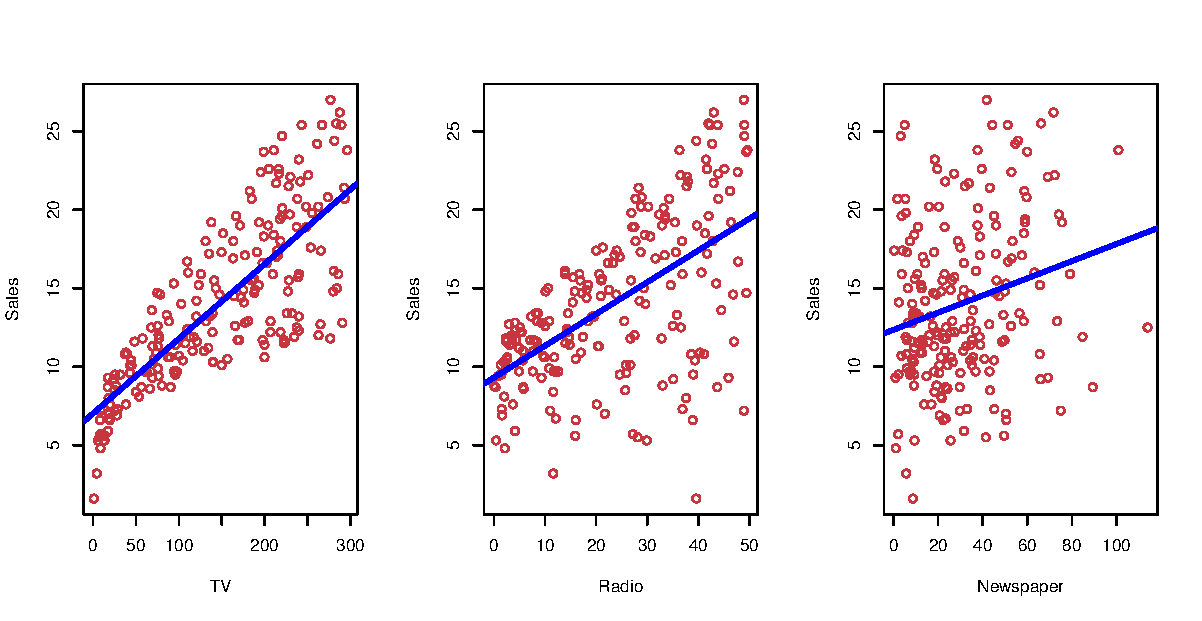
\includegraphics[width=0.6\textwidth]{2_1}
	\end{center}
	\vspace{-5mm}
	\begin{itemize}
		\item The plots display \dat{sales} as a function of the advertising budgets.
		\item Each plot is a \emph{scatter plot} of \dat{sales} versus a budget.
		\item We have overlaid a \emph{least squares line} fit on each plot.
	\end{itemize}
	\bottomline{We can already spot some promising relationships.}
\end{frame}

\begin{frame}{Example: Advertising}
	\begin{itemize}
		\item The advertising budgets are \e{input variables}.
		\item We denote the input variables with $X$.
		\item We use subscripts to distinguish them.
		\item For example, $X_1$ = \dat{TV}, $X_2$ = \dat{radio}, $X_3$ = \dat{newspaper}.
		\item The input variables are also called \e{predictors}, \e{independent variables}, \\
			\e{features} or simply \e{variables}.
		\item \dat{sales} is the \e{output variable}.
		\item Output variables are also called \e{dependent variables} or \e{responses}.
		\item We denote the output variables with $Y$.
	\end{itemize}
	\bottomline{Don't get confused by different names.}
\end{frame}

\begin{frame}{Models}
	\begin{itemize}
		\item Suppose we observe a \e{quantitative} response $Y$,\\
			and $p$ different predictors, $X_1, X_2, \dots X_p$. 
		\item We assume that there is some relationship between $Y$ and $X$.
		\item We can write this in the very general form
			\[ Y = f(X) + \epsilon\]
		\item Here $f$ is a fixed but unknown function of $X = (X_1, X_2, \dots, X_p)$.
		\item And $\epsilon$ is a random error term, independent of $X$ with mean zero.
		\item We say $f$ represents the \e{systematic} information\\
			that $X$ provides about $Y$.
	\end{itemize}
	\bottomline{This is the most general form of a \e{model}.}
\end{frame}

\begin{frame}{Example: Income}
	\vspace{-5mm}
	\begin{center}
		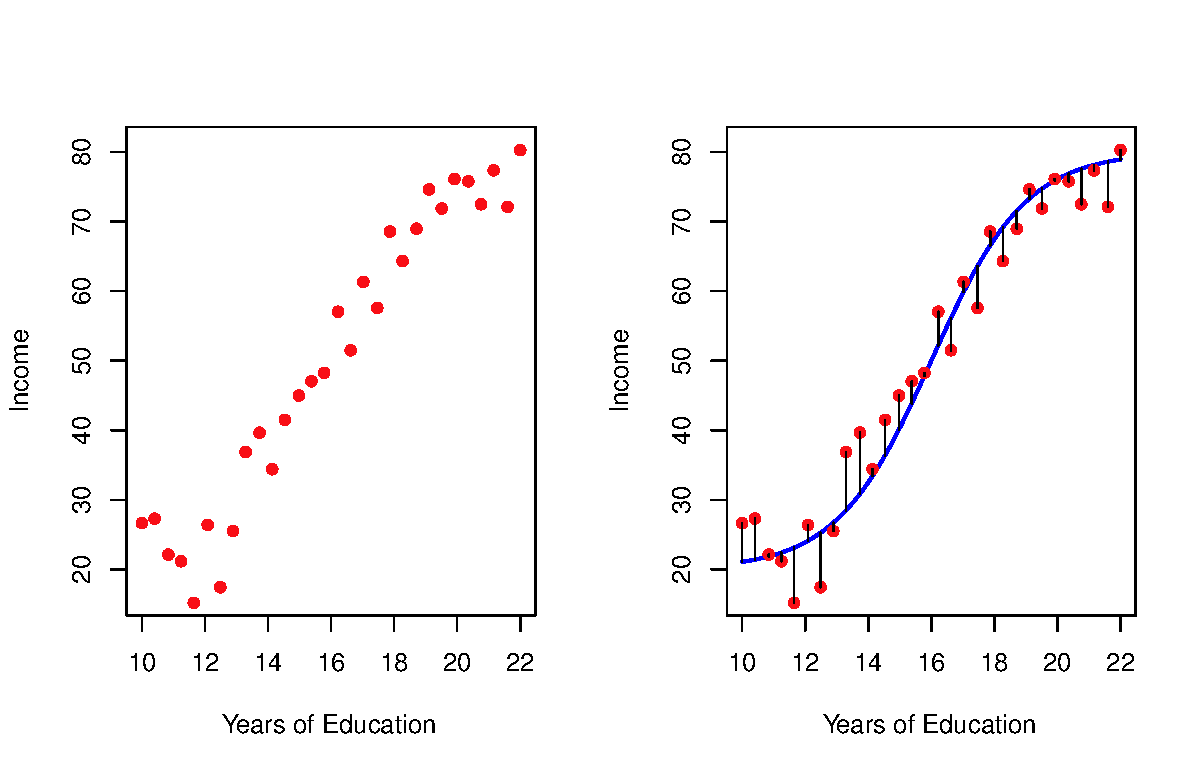
\includegraphics[width=0.5\textwidth]{2_2}
	\end{center}
	\vspace{-5mm}
	\begin{itemize}
		\item The figure shows a scatter plot of \dat{income} versus \dat{years of education}.
		\item The blue curve is the true functional relationship $f(X) =f(X_1)$.
		\item The vertical lines represent the error terms $\epsilon$.
	\end{itemize}
	\bottomline{This is a simulated data set.}
\end{frame}

\begin{frame}{Example: Income}
	\vspace{-5mm}
	\begin{center}
		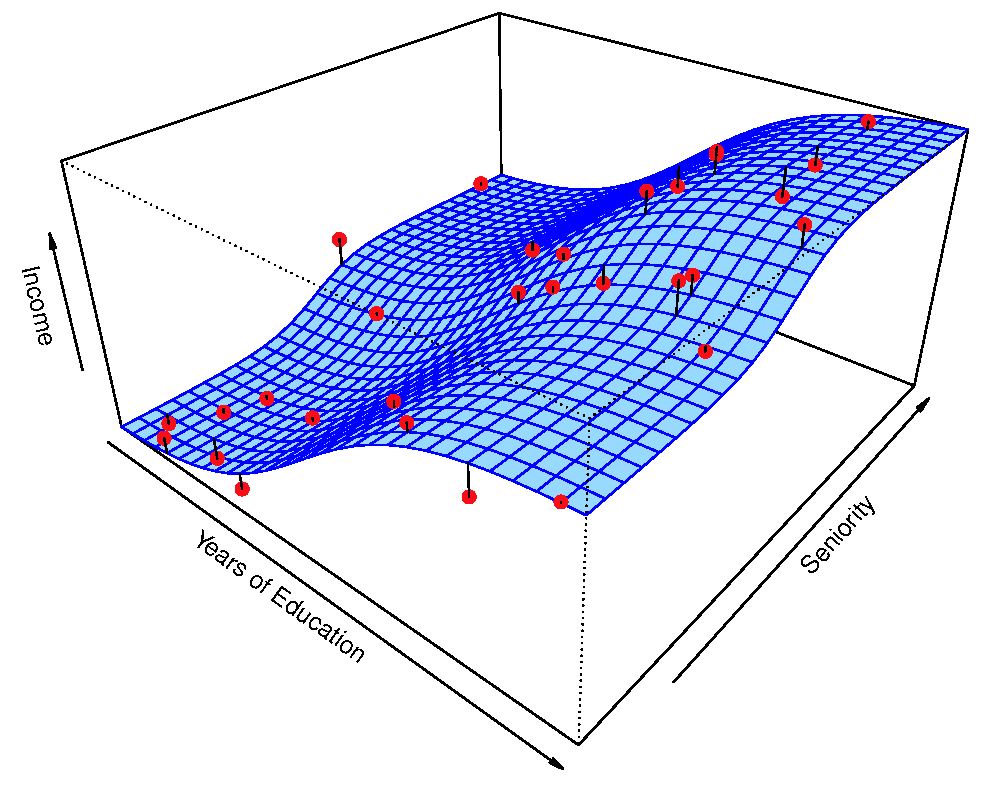
\includegraphics[width=0.4\textwidth]{2_3}
	\end{center}
	\vspace{-5mm}
	\begin{itemize}
		\item The figure shows a 3D scatter plot of \dat{income} versus \dat{years of education}
			and \dat{seniority}.
		\item The blue surface is the true functional relationship $f(X) = f(X_1, X_2)$.
		\item The vertical lines represent the error terms $\epsilon$.
	\end{itemize}
	\bottomline{Visualising higher dimensions is hard.}
\end{frame}

\begin{frame}{What is Statistical Learning?}
	\begin{blurb}
		In essence, statistical learning refers to to a set of approaches for estimating
		the function $f$.

		In this lecture we cover the key theoretical concepts that arise in estimating $f$, as well
		as techniques for evaluating the estimates obtained.
	\end{blurb}
	\bottomline{This equally applies to machine learning.}
\end{frame}

\begin{frame}{Why estimate $\bm{f}$?}
	%\begin{itemize}
		%\item There are two main reasons why we wish to estimate $f$.
	%\end{itemize}
		There are two main reasons why we wish to estimate $f$.
	\begin{enumerate}
		\item \e{Prediction}: assuming the inputs $X$ are readily available, we simply want ot
			predict
			\[\hat{Y} = \hat{f}(X)\]
			without being interested in the exact form of $\hat{f}$.
		\item \e{Inference}: we want to understand the functional relationship
			\[Y = Y(X_1, X_2, \dots, X_p)\]
			between the predictors and the response.
	\end{enumerate}
	\bottomline{We discuss each in more detail.}
\end{frame}

\begin{frame}{Prediction}
	\begin{itemize}
		\item Often the inputs $X$ are readily available but the response $Y$ is not.
		\item Since the error term $\epsilon$ averages to zero, we can then predict
			\[\hat{Y} = \hat{f}(X)\]
			where $\hat{f}$ represents the estimate of $f$ and $\hat{Y}$ is the resulting
			prediction of $Y$.
		\item In this scenario we are not interested in the exact form of $\hat{f}$.
		\item We are mostly concerned with the accuracy of $\hat{Y}$.
	\end{itemize}
	\bottomline{Here $\bm{\hat{f}}$ is often treated as a \e{black box}. But we don't have to!}
\end{frame}

\begin{frame}{Prediction Accuracy}
	\begin{itemize}
		\item The accuracy of $\hat{Y}$ depends on two quantities:
			\begin{enumerate}
				\item the \e{reducible error}
				\item the \e{irreducible error}
			\end{enumerate}
		\item The reducible error is due to $\hat{f}$ not being a perfect estimate of $f$.\\
			(We can potentially come up with better statistical learning techniques to 
			improve $\hat{f}$).
		\item Even if our estimate of the relationship was perfect ($\hat{f} = f$),\\
			our estimate $\hat{Y}$ would still have an error!
		\item This irreducible error is due to our \e{observations} not being perfect.\\
			(The error term $\epsilon$).
	\end{itemize}
	\bottomline{You have to understand what you can improve and what you can't.}
\end{frame}

\begin{frame}{Prediction Accuracy}
	\begin{itemize}
		\item Assuming that $\hat{f}$ and $X$ are fixed, we can show that
			\begin{align*}
				E[(Y - \hat{Y})^2] &= E[(f(X) + \epsilon - \hat{f}(X))^2]\\ 
				&= \underbrace{E[(f(X) - \hat{f}(X))^2]}_\text{Reducible}
				+ \underbrace{\text{Var}(\epsilon)}_\text{Irreducible} \\ 
			\end{align*}
			where $E[(Y - \hat{Y})^2]$ is the average, or \e{expected value}, of the squared\\
			difference between the predicted and the true value of $Y$,\\
			and $\text{Var}(\epsilon)$ is the \e{variance} of the error term $\epsilon$.
		\item The average, or expected value, $E[z]$ is often written as $\overline{z}$ or $\langle z \rangle$.
		\item The variance is then $\text{Var}(z) = \langle (z - \overline{z})^2 \rangle
			= \langle z^2 \rangle - {\langle z \rangle}^2 = \overline{z^2} - \overline{z}^2$.
	\end{itemize}
	\bottomline{All techniques we learn aim to estimate $\bm{f}$ while minimising the reducible error.}
\end{frame}

\begin{frame}{Inference}
	\begin{itemize}
		\item We are often interested in \e{how} $X_1, X_2, \dots, X_p$ affect $Y$.
		\item We want to estimate $f$, but not necessarily predict $Y$.
		\item The aim is to understand the \e{functional relationship} between $Y$ and $X$.
	\end{itemize}
	\bottomline{We can \e{not} treat $\bm{\hat{f}}$ as a black box in this scenario.}
\end{frame}

\begin{frame}{Inference: Questions}
	\begin{cpage}
		\begin{itemize}
			\item \e{\orange Which predictors are associated with the response?}\\
				We want to identify the \e{important} predictors.
			\item \e{\orange What is the relationship between the response and each predictor?}\\
				For example, predictors can have positive or negative influence\\
				on the response. Any functional relationship can occur, 
				possibly depending on the values of the other predictors.
			\item \e{\orange Can the relationship between $Y$ and each predictor be summarised as
				a linear equation?}\\
				It greatly simplifies things when the relationship can be captured by a linear model.
				Historically, models have been mostly chosen to be linear. However, the true relationships
				are very rarely linear.
		\end{itemize}
	\end{cpage}
	\bottomline{Linear is good, but rarely true.}
\end{frame}

\begin{frame}{How do we estimate $\bm{f}$?}
	\begin{columns}
		\begin{column}{0.7\textwidth}
			\begin{itemize}
				\item We have $n$ \e{observations} of $X$ and $Y$.
				\item In the plots on the right $n$ is 30.
				\item This is the \e{training data}.
				\item We use these observations to \e{train}, or \e{teach}, our model\\
					how to estimate $f$.
				\item The goal is to find a function $\hat{f}$ such that $Y \approx \hat{f}(X)$,
					for each observation $(X, Y)$.
			\end{itemize}
		\end{column}
		\begin{column}{0.3\textwidth}
			\begin{center}
				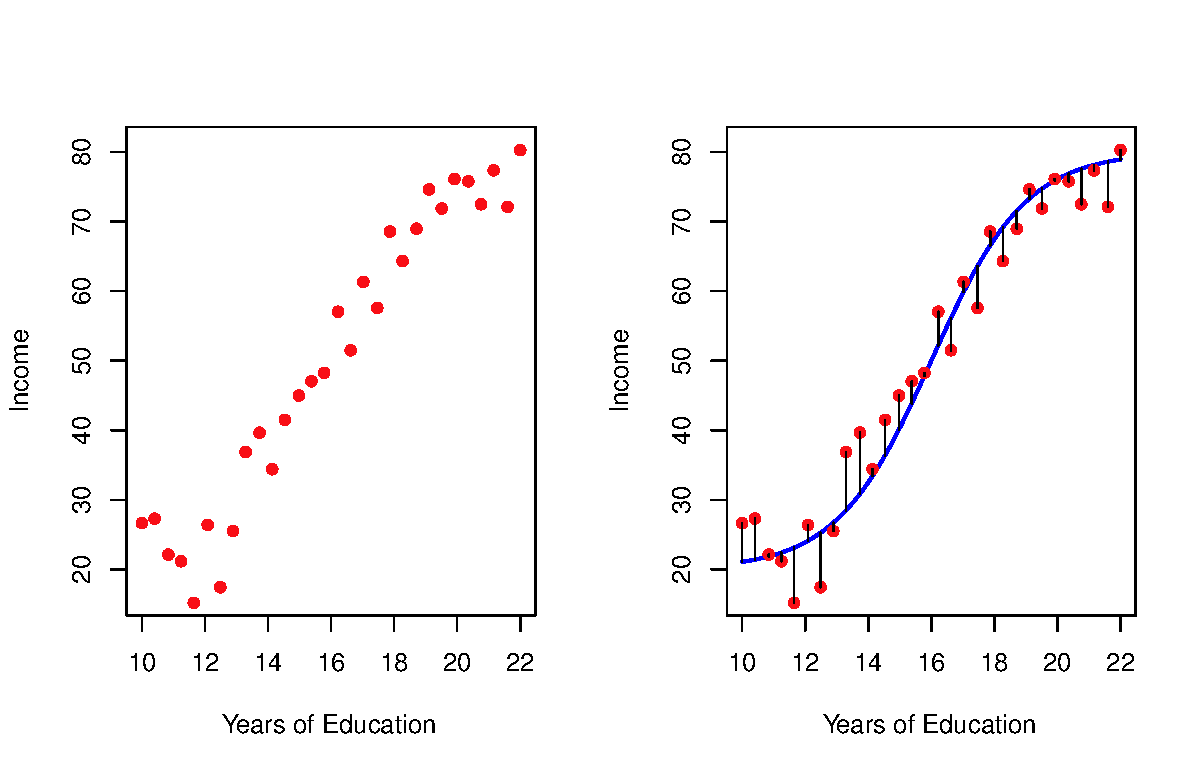
\includegraphics[width=\textwidth]{2_2}
			\end{center}
			\begin{center}
				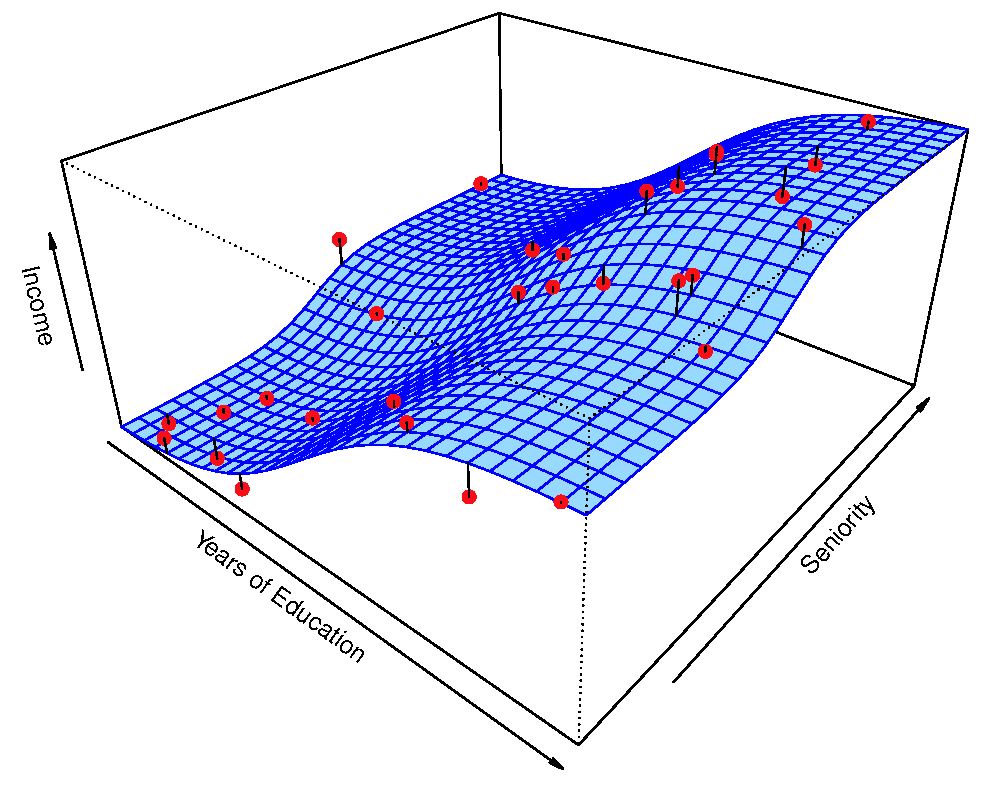
\includegraphics[width=0.9\textwidth]{2_3}
			\end{center}
		\end{column}
	\end{columns}
	\bottomline{Statistical learning methods are either \e{parametric} or \e{non-parametric}.}
\end{frame}

\begin{frame}{Parametric Methods}
	\begin{cpage}
		\begin{enumerate}
			\item \e{\orange Make an assumption about the functional form of $f$.}\\
				A very simple assumption is a linear model:
				\[ f(X) = \beta_0 + \beta_1 X_1 + \beta_2 X_2 + \dots + \beta_p X_p\]
				With a linear model we only need to estimate $p + 1$ parameters. 
				We will cover linear models in great detail in the next lecture.
			\item \e{\orange Use the training data to train, or fit, the model.}\\
				For a linear model we need to estimate the parameters 
				$\beta_0, \beta_1, \beta_2, \dots, \beta_p$ such that:
				\[ Y \approx \hat{\beta}_0 + \hat{\beta}_1 X_1 + \hat{\beta}_2 X_2 
				+ \dots + \hat{\beta}_p X_p \] 
		\end{enumerate}
	\end{cpage}
	\bottomline{Non-linear models are of course possible, but harder to fit.}
\end{frame}

\begin{frame}{Linear Model Example}
	\vspace{-5mm}
	\begin{center}
		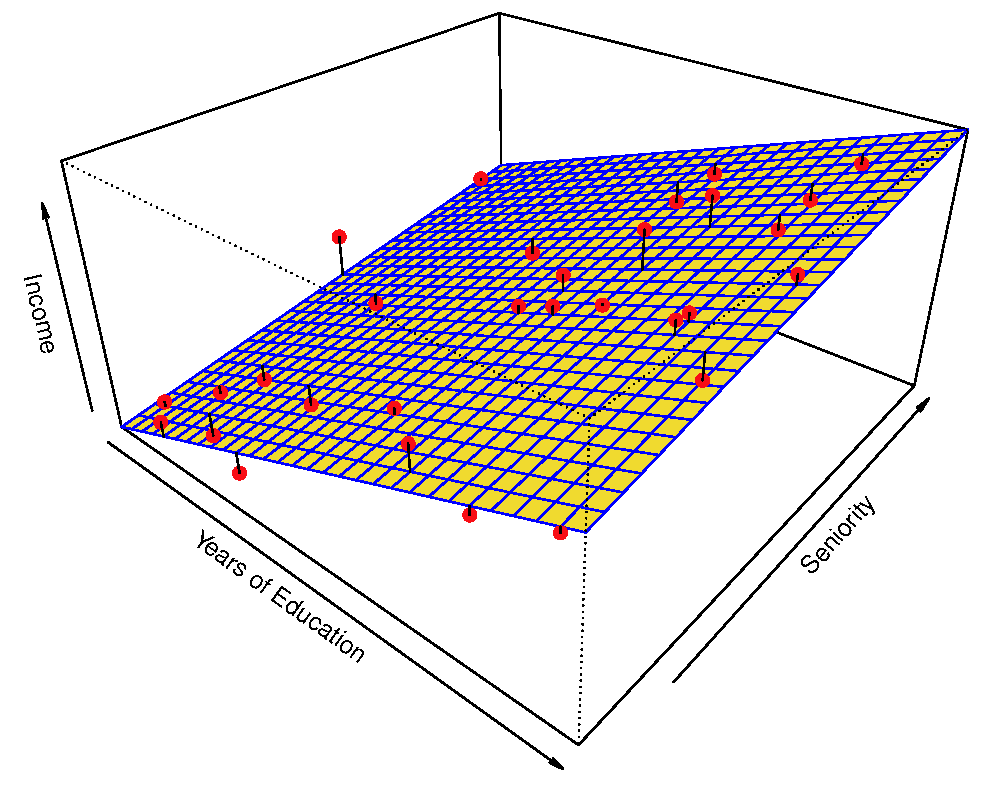
\includegraphics[width=0.5\textwidth]{2_4}

		\[ \text{\dat{income}} \approx \hat{\beta}_0 
			+ \hat{\beta}_1\times\text{\dat{years of education}}
		+ \hat{\beta}_2\times\text{\dat{seniority}}\]
	\end{center}
\end{frame}

\begin{frame}{Non-parametric Methods}
	\begin{cpage}
		\begin{enumerate}
			\item \e{\orange No assumption about the functional form of $f$ is made.}\\
			\item \e{\orange Seek an estimate of $f$ that smoothly approaches the data points\\
				in the training data.}
		\end{enumerate}
		\begin{itemize}
			\item[$+$] Avoids choosing potentially very wrong models.
			\item[$+$] Can approximate complex functional relationships.
			\item[$-$] Often needs many more observations for the fit.
			\item[$-$] Prone to over-fitting.
		\end{itemize}
	\end{cpage}
	\bottomline{Oddly, non-parametric methods can have a lot of parameters.}
\end{frame}

\begin{frame}{Non-parametric Example}
	\vspace{-5mm}
	\begin{center}
		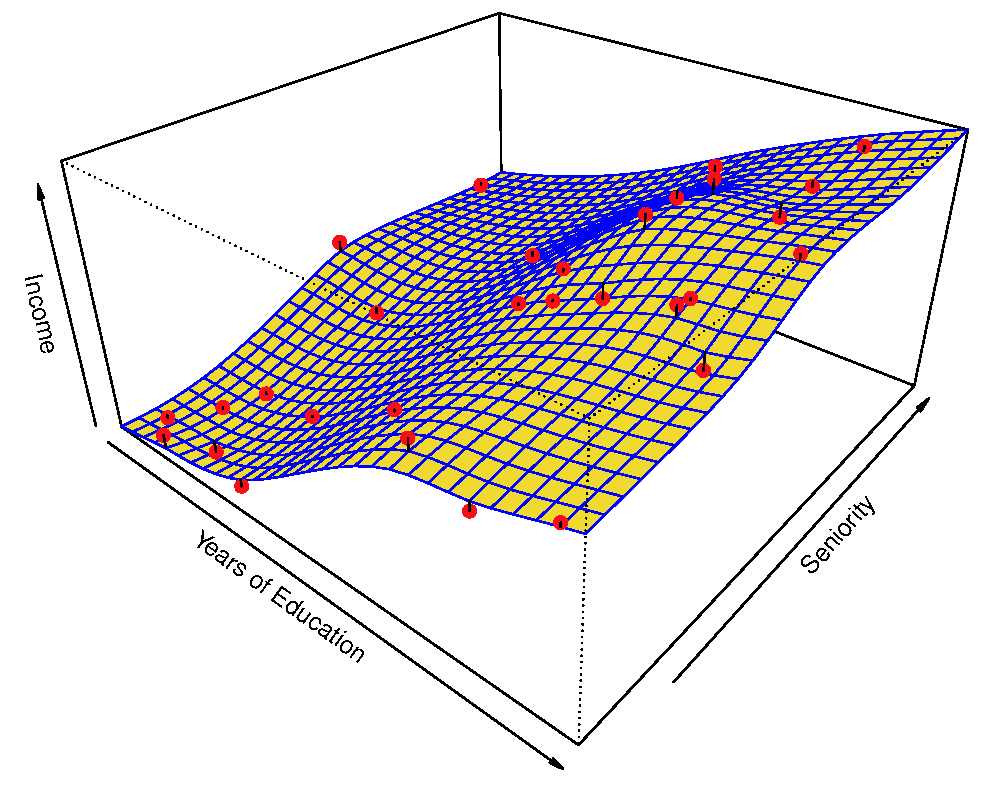
\includegraphics[width=0.5\textwidth]{2_5}

		Approximation to $f$ to predict \dat{income} using a \e{thin-plate spline}. 
	\end{center}
	\bottomline{Better fit to the training data than the linear model.}
\end{frame}

\begin{frame}{Non-parametric Example}
	\vspace{-5mm}
	\begin{center}
		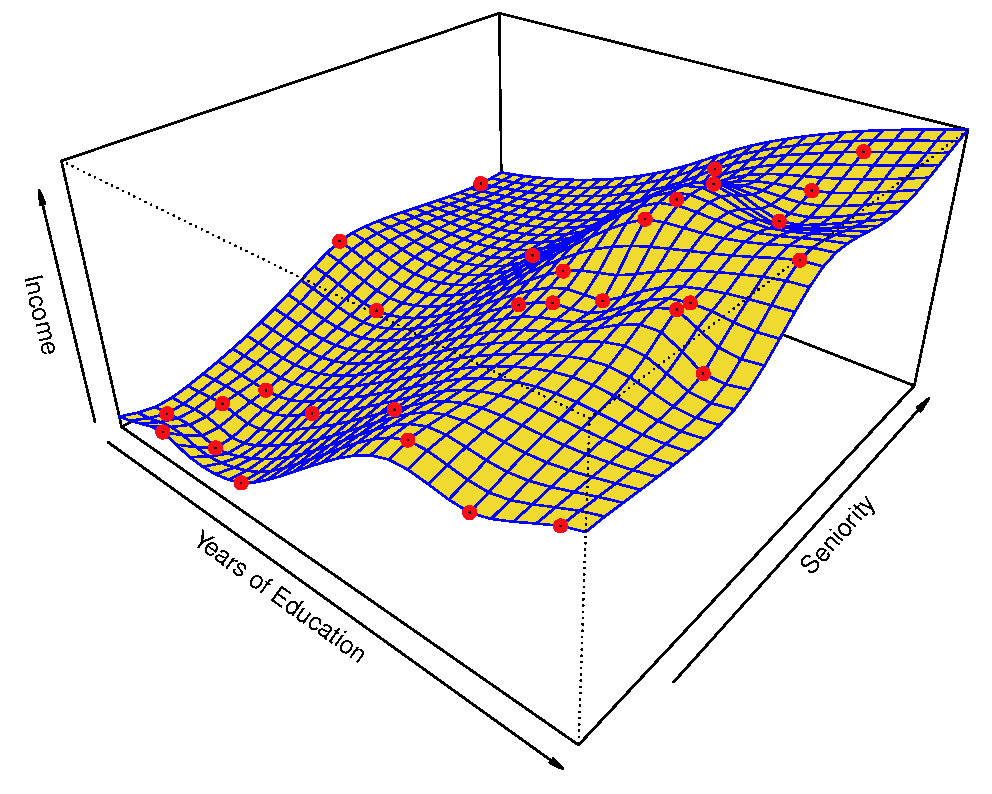
\includegraphics[width=0.5\textwidth]{2_6}

		A less smooth spline fit that fits the training data perfectly. 
	\end{center}
	\bottomline{This is an example of \e{over-fitting}!}
\end{frame}

\begin{frame}{Accuracy versus Interpretability Trade-off}
	\begin{cpage}
		\begin{itemize}
			\item[] \e{\orange Why would we choose a less flexible approach?}
			\item Interpretability is often desirable (inference).
			\item For example, in a linear model we can directly infer whether\\
				a relationship is positive or negative from the sign of\\
				the $\beta$ coefficient.
			\item[] \e{\orange Why would we choose a more flexible approach?}
			\item We might be mostly interested in the accuracy of\\
				our estimate of $f$ (prediction).
			\item In the extreme, this is a \e{black box} approach where we don't care about
				the interpretation at all.
		\end{itemize}
	\end{cpage}
	\bottomline{This is a \e{trade-off}, we have to decide.}
\end{frame}

\begin{frame}{Accuracy versus Interpretability Trade-off}
	\vspace{-5mm}
	\begin{center}
		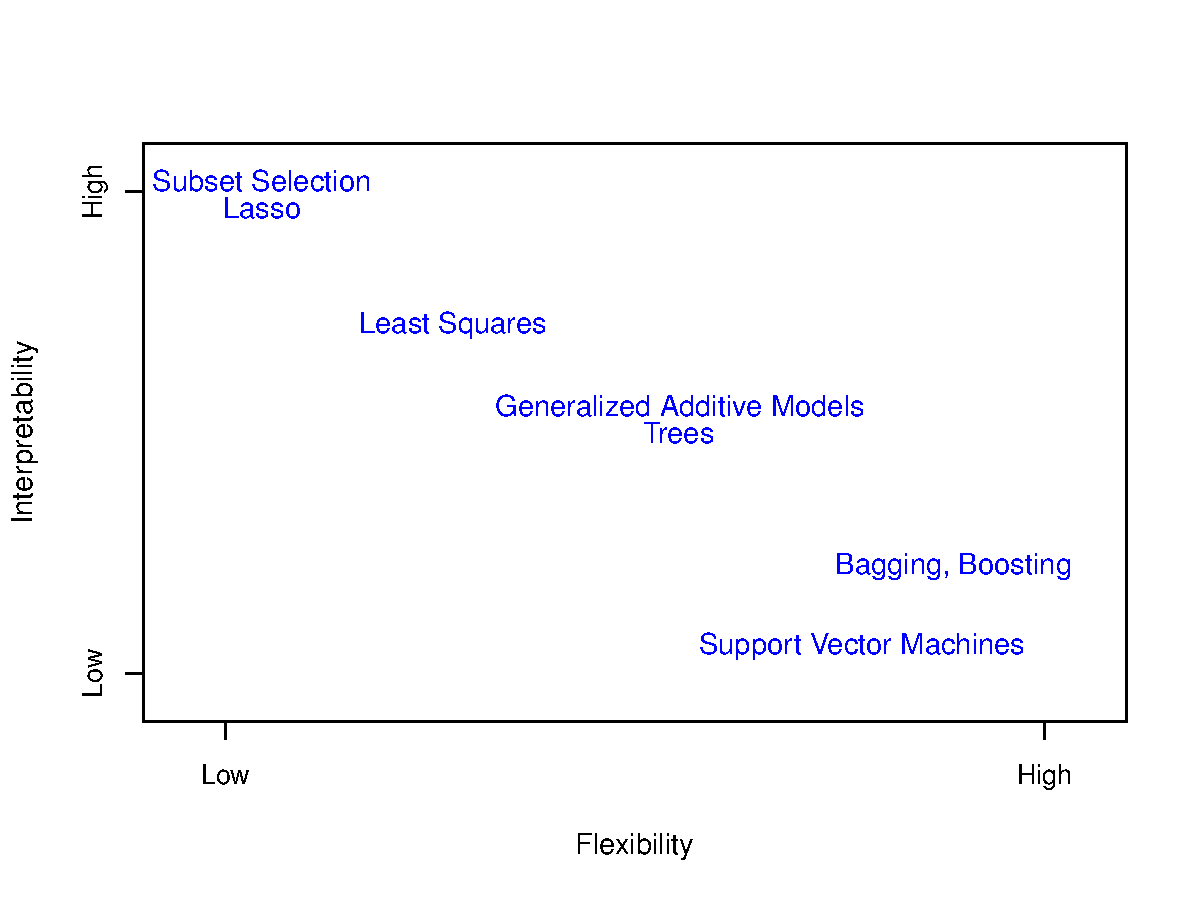
\includegraphics[width=0.6\textwidth]{2_7}

		In general, more flexible statistical learning methods have lower interpretability.
	\end{center}
	\bottomline{We'll learn more about the methods mentioned in the plot later.}
\end{frame}

\begin{frame}{Supervised versus Unsupervised Learning}
	\begin{cpage}
		\begin{itemize}
			\item[] \e{\orange Supervised Learning}
			\item We have $n$ observations of the $p$ predictors $X_j$ \e{and}
				the corresponding response $Y$.
			\item In this case we can fit a model to the training data.
			\item The \e{supervision} comes in through the presence of the known
				response $Y$ in the training data.
			\item[] \e{\orange Unsupervised Learning}
			\item We have $n$ observations of the $p$ predictors $X_j$,
				but \e{no access} to the corresponding response $Y$ in the training data.
			\item All we can do is look for \e{patterns} in the training data.
		\end{itemize}
	\end{cpage}
	\bottomline{This distinction is not always clear-cut.}
\end{frame}

\begin{frame}{Unsupervised Example}
	\vspace{-5mm}
	\begin{center}
		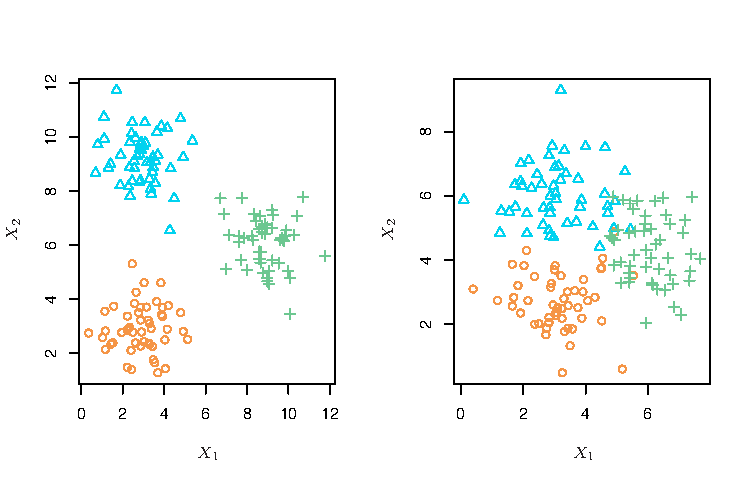
\includegraphics[width=0.6\textwidth]{2_8}

		Clustering data involving three groups. Left: little overlap. Right: larger overlap.
	\end{center}
	\bottomline{We need to automate this for large data sets.}
\end{frame}

\begin{frame}{Regression versus Classification}
	\begin{itemize}
		\item Variables, in particular responses, can be \e{quantitative} or
			\e{qualitative}.
		\item[] \e{\orange Quantitative Responses -- Regression Problems}
		\item Gas mileage, crime rate, sales. 
		\item[] \e{\orange Qualitative Responses -- Classification Problems}
		\item Sex (male, female), default on debt (yes, no), brand (Apple, Samsung, Blackberry).
	\end{itemize}
	\bottomline{In terms of statistical learning methods the distinction is not crisp.}
\end{frame}

\begin{frame}{Assessing Model Accuracy}
	\begin{itemize}
		\item In this course we introduce a wide range of statistical learning methods.
		\item Why are we doing this?
		\item Why not just teach the \e{best} method?
		\item No single method dominates all others over all possible data sets.
		\item It is \e{our} task to decide which method produces the best results on
			a given data set.
		\item We therefore need a way to \e{measure} how well we are doing.
	\end{itemize}
	\bottomline{There is no free lunch in statistical learning.}
\end{frame}

\begin{frame}{Measuring Fit Quality}
	\begin{itemize}
		\item How can we measure the quality of a fit?
		\item We need to quantify how close our estimate $\hat{Y} = \hat{f}(X)$ is to the
			true values $Y$.
		\item Clearly, the difference between the two is a measure of this,\\
			but we don't care about the sign.
		\item We therefore use the \e{mean squared error}, MSE:
			\[ 
				\text{MSE} = \frac{1}{n}\sum_{i=1}^n (y_i - \hat{f}(x_i))^2
				= E[(Y - \hat{f}(X))^2]
				= \langle (Y - \hat{f}(X))^2 \rangle 
			\]
	\end{itemize}
	\bottomline{Other choices for the \e{loss function} are possible. This is the most straight-forward and common choice.}
\end{frame}

\begin{frame}{Measuring Fit Quality}
	\begin{itemize}
		\item We could simply compute the MSE on the training data.
		\item Most fit, or learning, methods work by minimising the MSE\\
			(or another suitable \e{loss function}) on the training data set.
		\item However, we want to make predictions on \e{future} observations,\\
			not available at the time of training.
		\item A better measure of how well we are doing is obtained by computing\\
			the MSE on a \e{test data set} that is \e{independent} of the training data set.
		\item We can always produce an independent test data set by only using a subset of 
			the available data for training and the remainder for testing (\e{cross validation}).
	\end{itemize}
	\bottomline{The MSE from the training data set overestimates the fit quality.}
\end{frame}

\begin{frame}{Measuring Fit Quality: Example 1}
	\vspace{-5mm}
	\begin{center}
		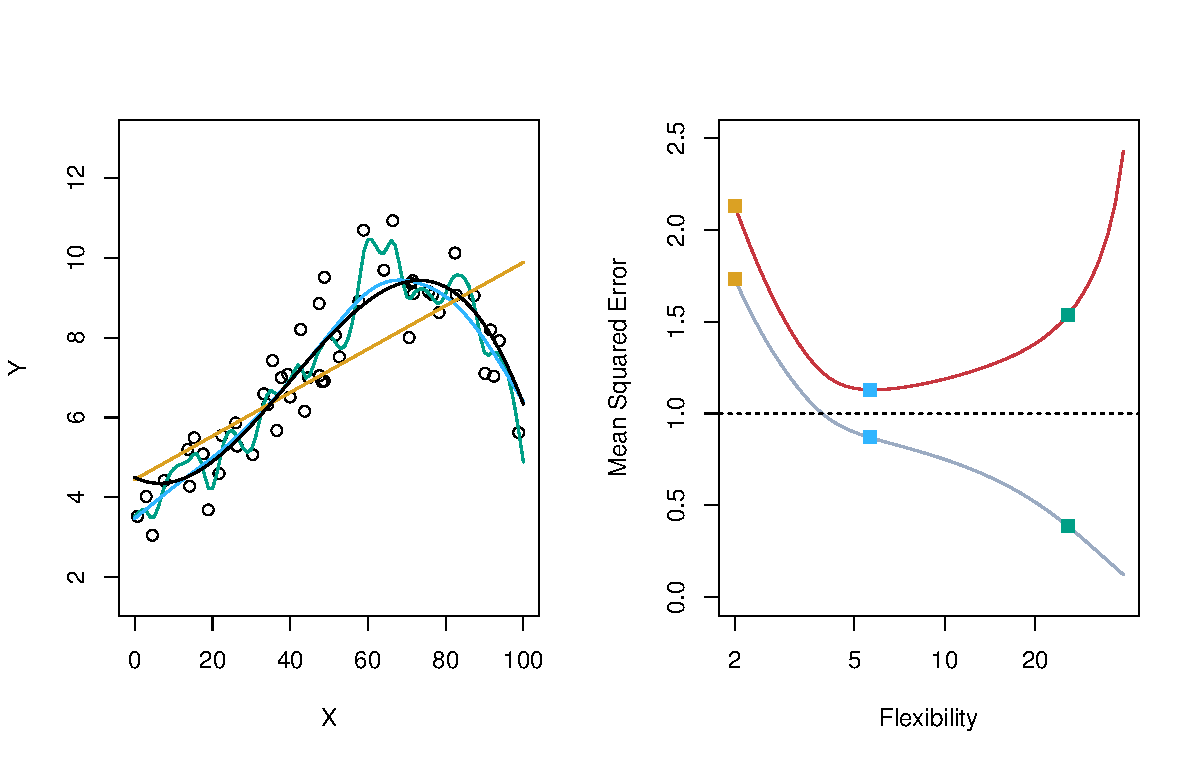
\includegraphics[width=0.6\textwidth]{2_9}

		Left: true $f$ (black), linear regression (orange), and spline fits (blue, green).\\
		Right: training (grey) and test (red) MSE.
	\end{center}
	\bottomline{The most flexible model over-fits the training data.}
\end{frame}

\begin{frame}{Measuring Fit Quality: Example 2}
	\vspace{-5mm}
	\begin{center}
		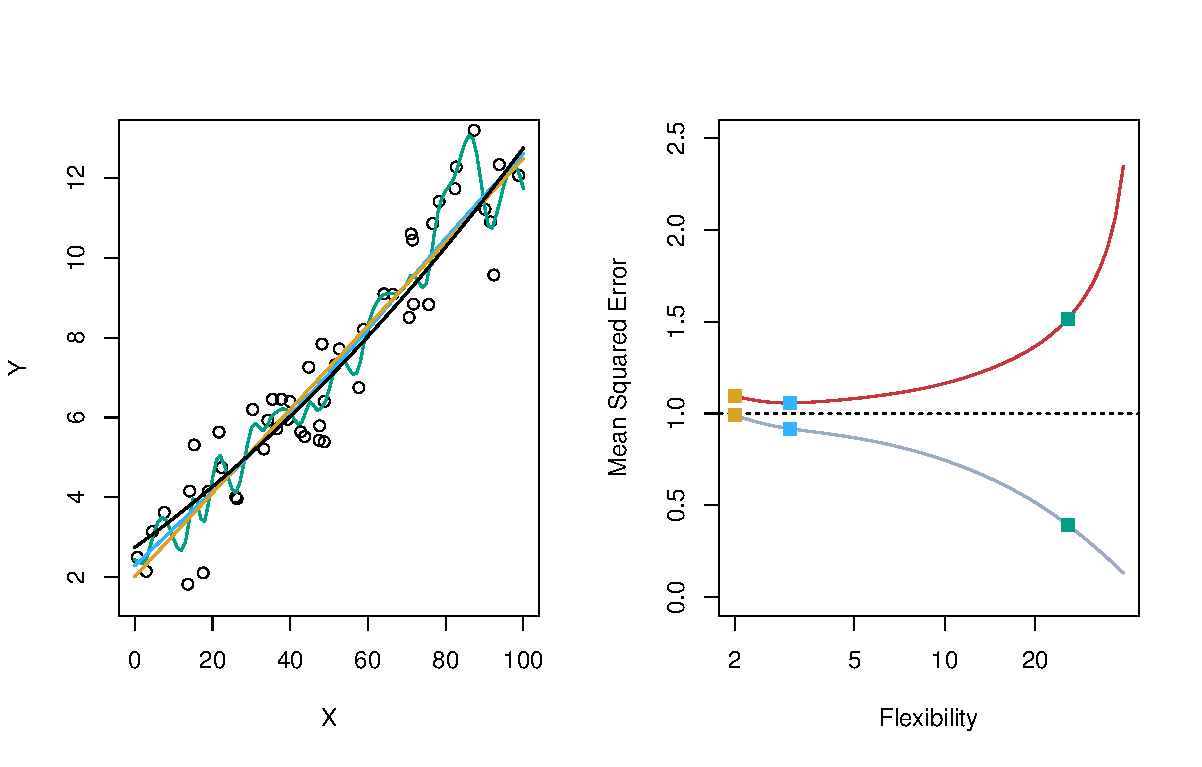
\includegraphics[width=0.6\textwidth]{2_10}

		Left: true $f$ (black), linear regression (orange), and spline fits (blue, green).\\
		Right: training (grey) and test (red) MSE.
	\end{center}
	\bottomline{The truth is more linear, so linear regression does well.}
\end{frame}

\begin{frame}{Measuring Fit Quality: Example 3}
	\vspace{-5mm}
	\begin{center}
		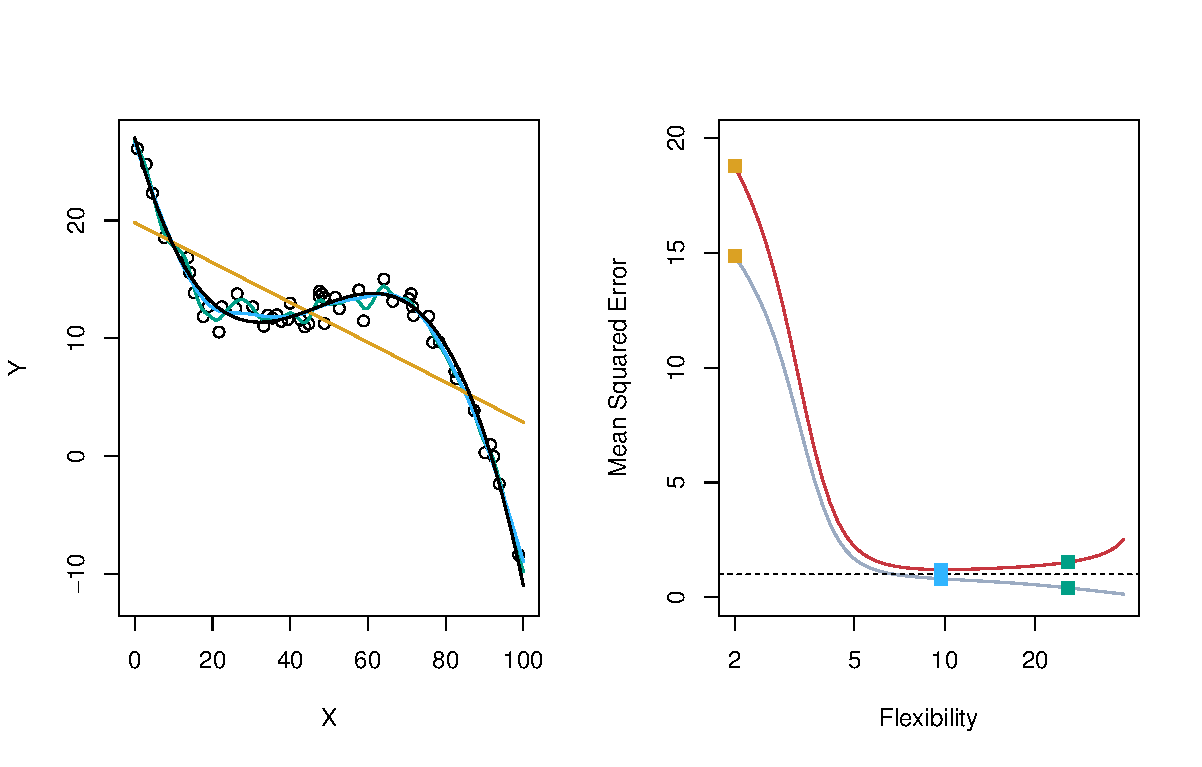
\includegraphics[width=0.6\textwidth]{2_11}

		Left: true $f$ (black), linear regression (orange), and spline fits (blue, green).\\
		Right: training (grey) and test (red) MSE.
	\end{center}
	\bottomline{The truth is highly non-linear, so linear regression does badly.}
\end{frame}

\begin{frame}{The Bias-Variance Trade-off}
	\begin{itemize}
		\item We denote the observations from a test data set as $(x_0, y_0)$.
		\item Then the test data set MSE is:
			\[ \text{MSE}_\text{test} = \langle (y_0 - \hat{f}(x_0))^2 \rangle \]
		\item We can then show that this can be decomposed like this:
			\[ 
			\langle (y_0 - \hat{f}(x_0))^2 \rangle
			= \underbrace{\text{Var}(\hat{f}(x_0)) + (\text{Bias}(\hat{f}(x_0))^2}_\text{Reducible} 
			+ \underbrace{\text{Var}(\epsilon)}_\text{Irreducible}
			\]
			where the \e{bias} is:
			\[ \text{Bias}(\hat{f}(x_0)) = \langle\hat{f}(x_0)\rangle - \langle f(x_0)\rangle\] 
	\end{itemize}
	\bottomline{In practice, we don't know the true $\bm{f}$ and can't compute the bias properly.}
\end{frame}

\begin{frame}{The Bias-Variance Trade-off}
	\begin{itemize}
		\item Given the test MSE
			\[ 
			\langle (y_0 - \hat{f}(x_0))^2 \rangle
			= \underbrace{\text{Var}(\hat{f}(x_0)) + (\text{Bias}(\hat{f}(x_0))^2}_\text{Reducible} 
			+ \underbrace{\text{Var}(\epsilon)}_\text{Irreducible}
			\]
			we want to minimize the variance of $\hat{f}(x_0)$ \e{and} the bias.
		\item This is often not possible at the same time.
		\item Highly flexible methods can eliminate the bias.
		\item That does \e{not} mean they perform better at prediction.
	\end{itemize}
	\bottomline{The bias-variance trade-off translates to a flexibility trade-off.}
\end{frame}

\begin{frame}{The Bias-Variance Trade-off}
	\vspace{-5mm}
	\begin{center}
		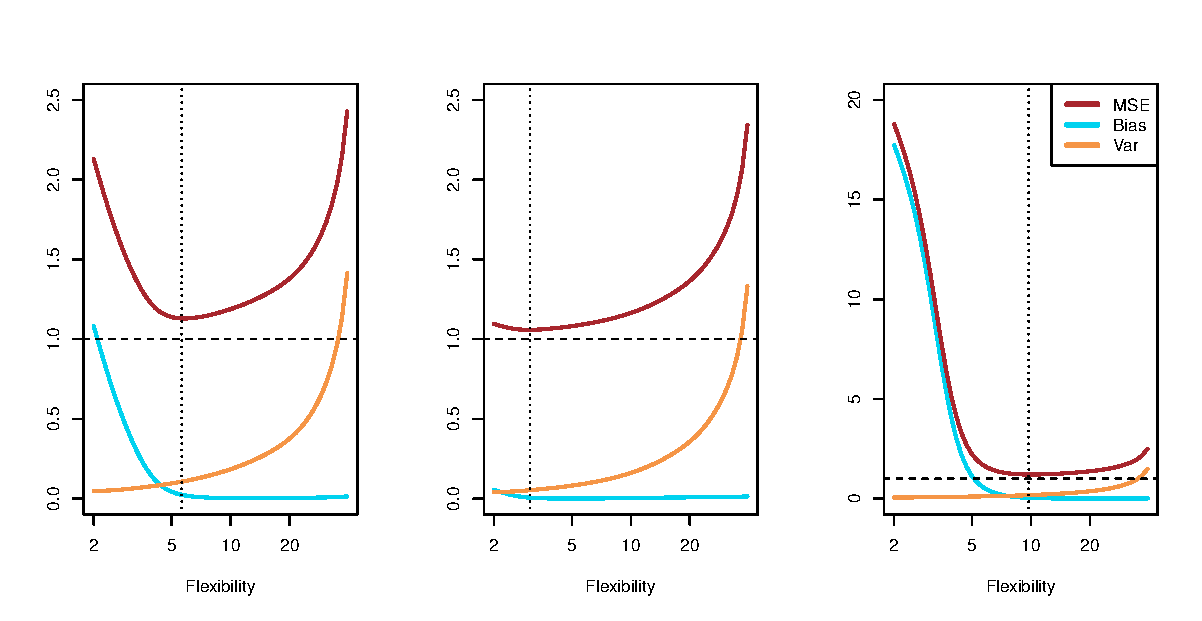
\includegraphics[width=0.8\textwidth]{2_12}

		The plots correspond to the three example data sets we have seen before.\\
		(Non-linear, almost linear, highly non-linear).
	\end{center}
\end{frame}

\begin{frame}{The Classification Setting}
	\begin{itemize}
		\item As before, we want to estimate $f$ from the training observations
			\[\lbrace (x_1, y_1), (x_2, y_2), \dots, (x_n, y_n) \rbrace\]
			and say we train a \e{classifier}.
		\item Now the responses $y_i$ are \e{qualitative}.
		\item That is, the $y_i$ are \e{labels} denoting the different \e{classes}
			the output variable can belong to.
		\item For example: 
			\[
				y = \text{\dat{origin}}, \text{\dat{origin}} 
				\in\lbrace \text{\dat{US}},\text{\dat{EU}},  \text{\dat{JP}} \rbrace
			\]  
	\end{itemize}
	\bottomline{Classifiers usually predict class \e{probabilities} from observations.}
\end{frame}

\begin{frame}{Probabilities}
	\begin{itemize}
		\item We need to formalise our notion of \e{probability.}
	\end{itemize}
	\begin{cpage}\orange
		We use probabilities to quantitatively express\\
		our relative believes in various propositions.
	\end{cpage}
	\begin{itemize}
		\item We can hear the mathematicians scream ``How can you formalise a \e{believe}?''.
		\item Some argue the whole notion is flawed and we can only ever speak of the \e{frequency}\\
			at which events occur in an \e{ensemble}.
		\item Of course, we often use observed frequencies to determine probabilities.
		\item But sometimes the concept of an ensemble does not make much sense.
		\item We take a pragmatic approach without getting too philosophical about it.
	\end{itemize}
	\bottomline{Don't get drawn into heated debates with hard-core frequentists.}
\end{frame}

\begin{frame}{Probabilities: Cook's Rules}
	\begin{itemize}
		\item We clearly need a \e{transitive} property: if we believe (a) more than (b)\\
			and (b) more than (c) then we must believe (a) more than (c).
			\[ P(a) > P(b) \land P(b) > P(c) \implies P(a) > P(c),\; P \in \R \]
		\item If we specify how much we believe $X$ to be true we have implicitly specified how much
			we believe $X$ to be false. With the conventional norm of one we write this as
			\[ P(X\vert I) + P(\bar{X}\vert I) = 1 \]
		\item If we specify how much we believe $X$ is true and then how much we believe\\
			$Y$ \e{given} $X$ is true, we have implicitly specified how much we believe $Y$ \e{and} $X$ are true.
			\[ P(Y, X\vert I) = P(Y\vert X, I) \times P(X\vert I) \]
	\end{itemize}
	\bottomline{These are the quantitative axioms necessary for logical and consistent reasoning.}
\end{frame}

\begin{frame}{Corollaries}
	\begin{itemize}
		\item[] \e{\orange Bayes' Theorem}
			\[
				P(Y\vert X, I) = \frac{P(X\vert Y, I)\times P(Y\vert I)}{P(X\vert I)}
			\]
	\end{itemize}
	\vspace{1cm}
	\begin{itemize}
		\item[] \e{\orange Marginalisation}
			\[
				P(Y\vert I) = \int_{-\infty}^{+\infty} P(Y, X\vert I) dX
			\]
	\end{itemize}
	\bottomline{Here $\bm{I}$ denotes our background knowledge and assumptions.}
\end{frame}

\begin{frame}{Bayes' Theorem}
	\begin{itemize}
		\item The power of Bayes' theorem is that it allows to turn one \e{conditional probability}\\
			into another.
		\item It relates $P(X\vert Y,I)$ to $P(Y\vert X,I)$.
		\item The importance of this is more obvious when we replace $Y$ with \e{hypothesis}\\
			and $X$ with \e{data}:
			\[
				P(\text{\e{\orange hypothesis}}\vert\text{\e{\blue data}}, I) \propto
				P(\text{\e{\blue data}}\vert\text{\e{\orange hypothesis}}, I) \times P(\text{\e{\orange hypothesis}}\vert I)
			\]
		\item Note that we have omitted the normalisation factor.
	\end{itemize}
	\bottomline{This relates the probability we are interested in to one we have a chance to measure!}
\end{frame}

\begin{frame}{Bayes' Theorem}
	\vspace{-5mm}
	\begin{center}
		\[
			P(Y\vert X, I) = \frac{P(X\vert Y, I)\times P(Y\vert I)}{P(X\vert I)}
		\]
	\end{center}
	\begin{popblock}{0.4\textwidth}{}
		\begin{tabular}[h]{ll}
			\e{\blue\bfseries Term} & \e{\blue\bfseries Name} \\
			$P(Y\vert X, I)$ & posterior probability \\
			$P(X\vert Y, I)$ & likelihood \\
			$P(Y\vert I)$ & prior probability \\
			$P(X\vert I)$ & evidence \\
		\end{tabular}
	\end{popblock}
	\bottomline{All statistical learning techniques are methods to approximate the posterior probability.}
\end{frame}

\begin{frame}{Classifier Accuracy}
	\begin{itemize}
		\item The concepts we have developed for regression also apply to classification.
		\item We need a way to quantify the accuracy of classifiers.
		\item We define the \e{training error rate}:
			\[
				\frac{1}{n}\sum^n_{i=1} I(y_i \ne \hat{y}_i)
				= \langle I(y_i \ne \hat{y}_i)\rangle,
				\;\;
				 I(y_i \ne \hat{y}_i) =
				 \begin{cases}
					 1 & y_i \ne \hat{y}_i \\
					 0 & y_i = \hat{y}_i \\
				 \end{cases}
			\]
		\item With the convention that $(x_0, y_0)$ denotes the test observations,\\
			the \e{test error rate is}:
			\[ \langle  I(y_0 \ne \hat{y}_0)\rangle \]
	\end{itemize}
	\bottomline{A good classifier minimises the test error rate.}
\end{frame}

\begin{frame}{The Bayes Classifier}
	\begin{itemize}
		\item The best possible classifier minimises the test error rate on average.
		\item It assigns each observation to the most likely class given the observed predictors.
		\item We write the probability of $Y$ belonging to class $j$, given the predictor\\
			observation $x_0$, as follows.
			\[ P(Y=j\vert X = x_0) \]
		\item In a scenario with two classes (say \dat{Up} and \dat{Down}) this classifier predicts\\
			$Y = \text{\dat{Up}}$ if
			\[ P(Y=\text{\dat{Up}}\vert X = x_0) > 0.5 \]
			and $Y = \text{\dat{Down}}$ otherwise.
		\item This is called the \e{Bayes Classifier} and it is ideal.
		\item On simulated data we can compute the above probability perfectly.
	\end{itemize}
	\bottomline{No method can do better than this proper Bayesian posterior probability.}
\end{frame}

\begin{frame}{The Bayes Decision Boundary}
	\vspace{-2mm}
	\begin{center}
		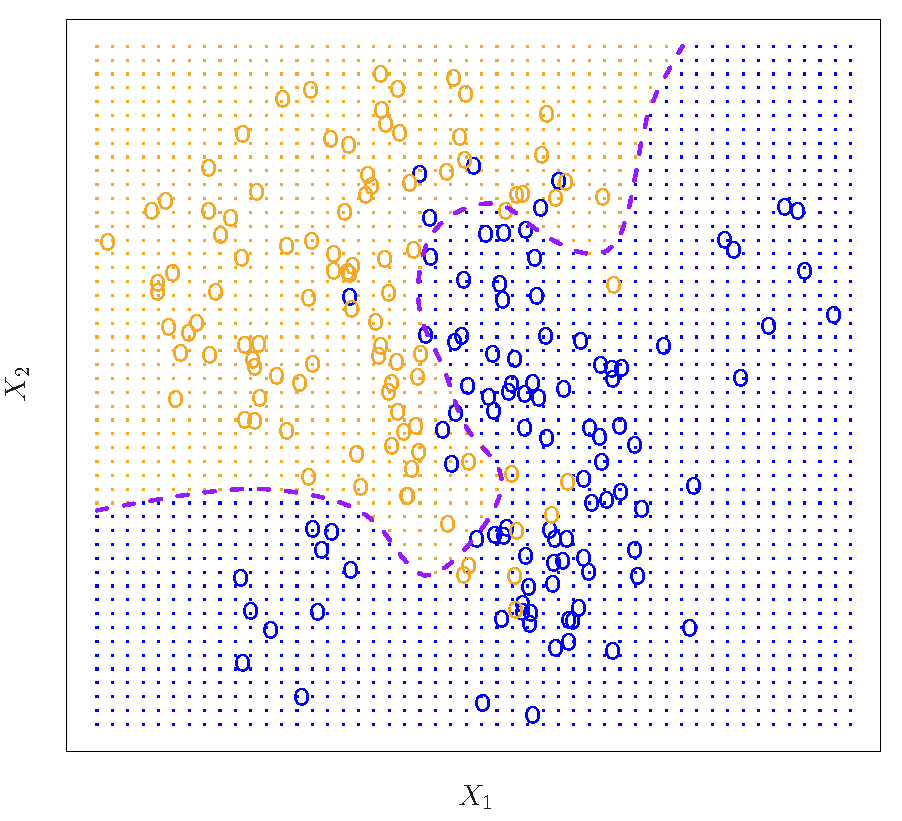
\includegraphics[width=0.45\textwidth]{2_13}

		A simulated data set with 100 observations. The dashed line is the \e{Bayes decision boundary}.
	\end{center}
\end{frame}

\begin{frame}{K-Nearest Neighbours}
	\begin{enumerate}
		\item Given an integer $K$ and a test observation $x_0$, find the $K$ observations $x_i$
			in the training data set that are closest to $x_0$, denoted by $\mathcal{N}_0$.
		\item Then estimate the conditional probabilities to observe $x_0$ from the relative frequencies\\
			of the classes in $\mathcal{N}_0$ (\e{likelihoods}):
			\[ P(X=x_0\vert Y=j) = \frac{1}{K}\sum_{i \in\mathcal{N}_0} I(y_i = j) \]
		\item Finally, use Bayes' theorem to compute the conditional \e{posterior probability}:
			\[P(Y=j\vert X=x_0) = \frac{P(X=x_0\vert Y=j)\times P(Y=j)}{P(X=x_0)}\]
	\end{enumerate}
	\bottomline{KNN \e{estimates} $\bm{P(Y\vert X)}$. The \e{flexibility} of KNN scales with $\bm{1/K}$.}
\end{frame}

\begin{frame}{K-Nearest Neighbours}
	\begin{center}
		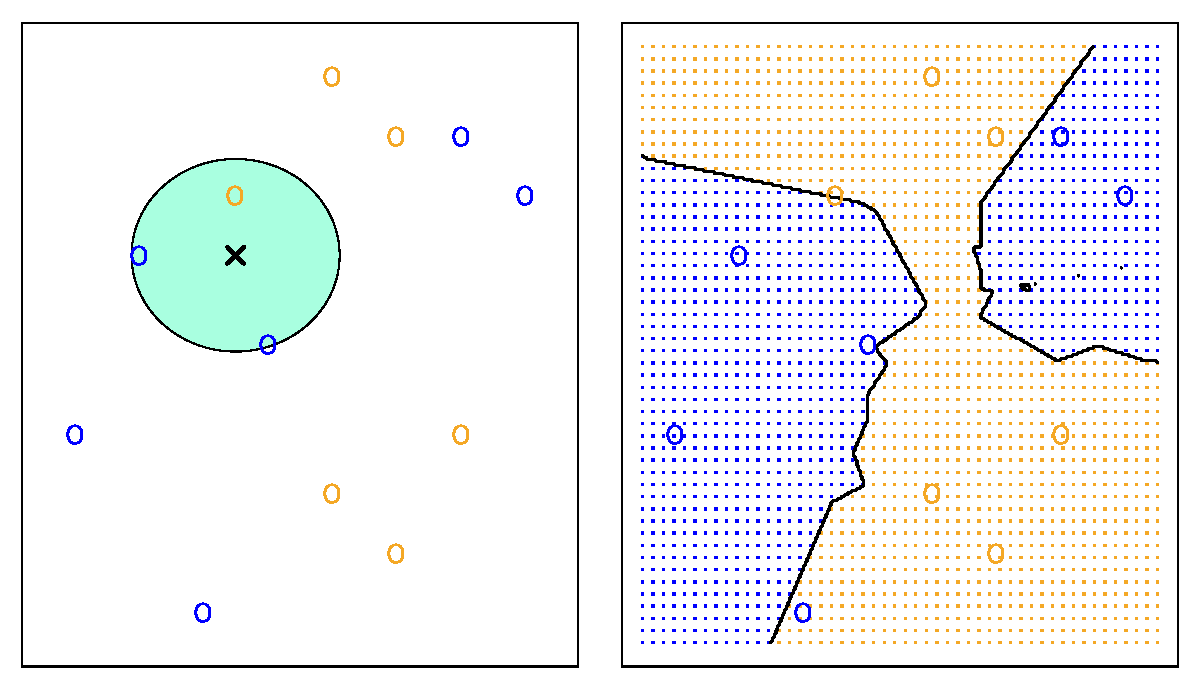
\includegraphics[width=0.7\textwidth]{2_14}

		The KNN approach with $K=3$. The black ``x'' in the left panel is a test observation.
	\end{center}
\end{frame}

\begin{frame}{K-Nearest Neighbours}
	\begin{center}
		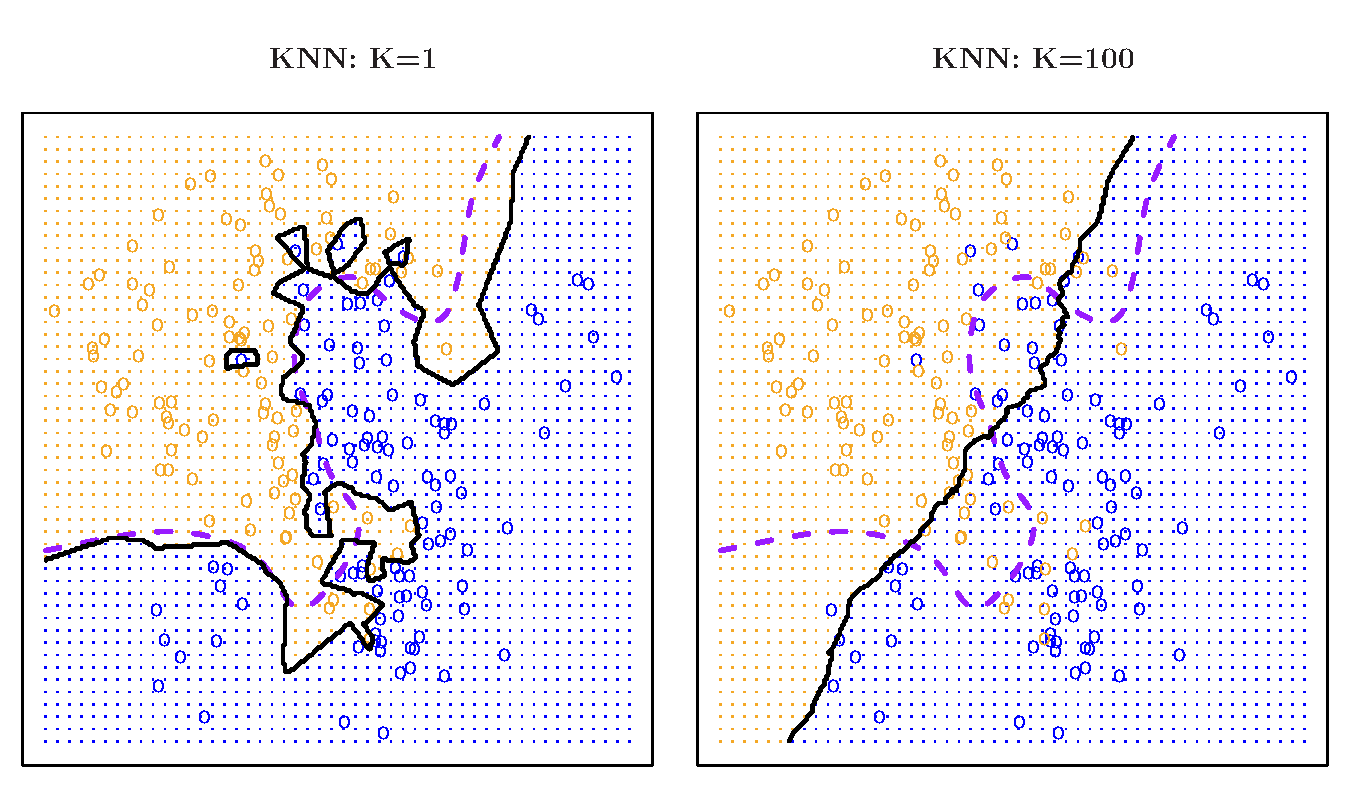
\includegraphics[width=0.7\textwidth]{2_16}

		A comparison of decision boundaries with $K=1$ and $K=100$. 
	\end{center}
\end{frame}

\begin{frame}{K-Nearest Neighbours}
	\begin{center}
		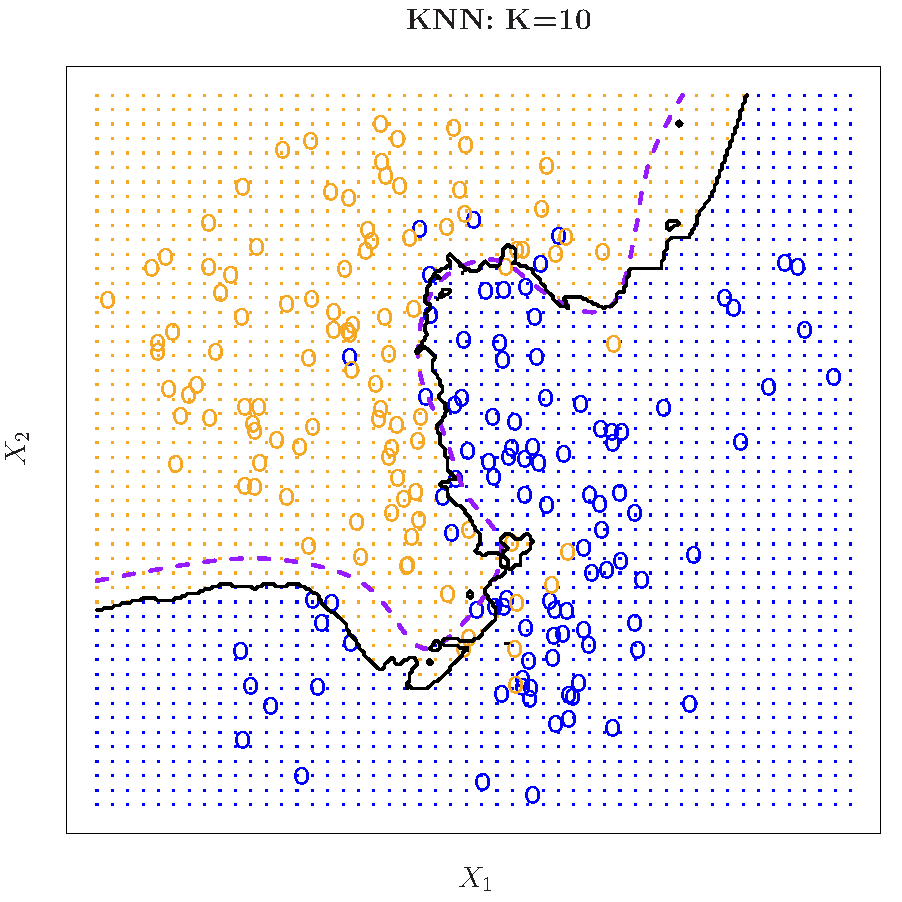
\includegraphics[width=0.4\textwidth]{2_15}

		Comparing to the Bayes decision boundary, $K=10$ seems a good choice. 
	\end{center}
\end{frame}

\begin{frame}{K-Nearest Neighbours}
	\begin{center}
		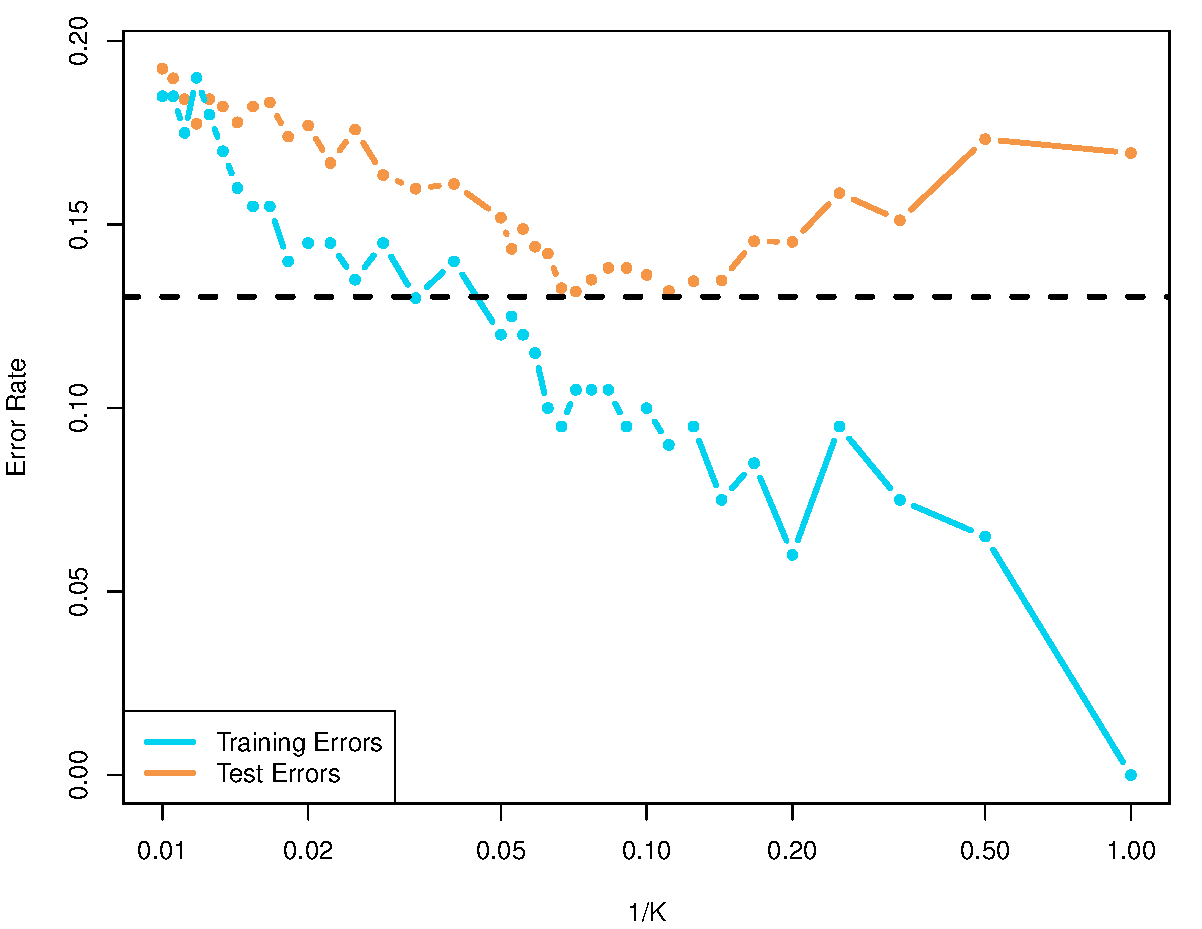
\includegraphics[width=0.5\textwidth]{2_17}

		Flexibility versus model performance on training and test data sets. 
	\end{center}
\end{frame}
\end{document}
